\subsection{Do changing scales explain deadline-specific weights?}

\label{sec:revision_scale}

The intermediate model preserves one nonnegative normalized direction while allowing a separate nonnegative amplitude and intercept at each deadline. It is fitted with three fixed initializations and a ridge penalty on the effective coefficients; all tuning remains inside the training folds. The separate model selects its penalty separately for each deadline.

The common-direction model reduces pooled MSE by 11.9--40.0\% relative to the common-coefficient fit. Allowing the direction also to change reduces MSE by another 24.3--36.1\% (Table~\ref{tab:revision_models}). Thus amplitude changes explain a substantial, preference-dependent part of the original gain, but do not account for it completely.

Of the 25 preference--deadline contrasts between the common-direction and separate models, 23 have positive lower bounds in the joint scenario-bootstrap simultaneous intervals over all 50 primary contrasts. These approximate intervals condition on the held-out predictions and do not include model-refitting uncertainty. A nonsignificant contrast is not evidence of equivalence; the declared exploratory margin is 0.001 absolute MSE.

\begin{table}[htbp]\centering\small\begin{tabular}{lrrrrrr}\toprule

Preference & Common & Scaled & Separate & B1 & B1+B3+B4 & Boosting\\\midrule

Equal & 0.02767 & 0.02000 & 0.01353 & 0.02245 & 0.01801 & 0.00962\\

Cost & 0.03985 & 0.03443 & 0.02371 & 0.03926 & 0.03015 & 0.01483\\

Direct thermal CO$_2$ & 0.03855 & 0.02315 & 0.01753 & 0.02397 & 0.02156 & 0.01275\\

Time & 0.01550 & 0.01366 & 0.00873 & 0.01838 & 0.01347 & 0.00682\\

Service & 0.03739 & 0.02385 & 0.01728 & 0.02546 & 0.02205 & 0.01260\\

\bottomrule\end{tabular}\caption{Nested held-out MSE over 3,000 observations per preference. Scaled denotes the common-direction model. B1 and the compact model have deadline-specific coefficients, as does boosting. These comparisons use the original five scenario folds of the weight study.}\label{tab:revision_models}\end{table}

\begin{figure}[htbp]\centering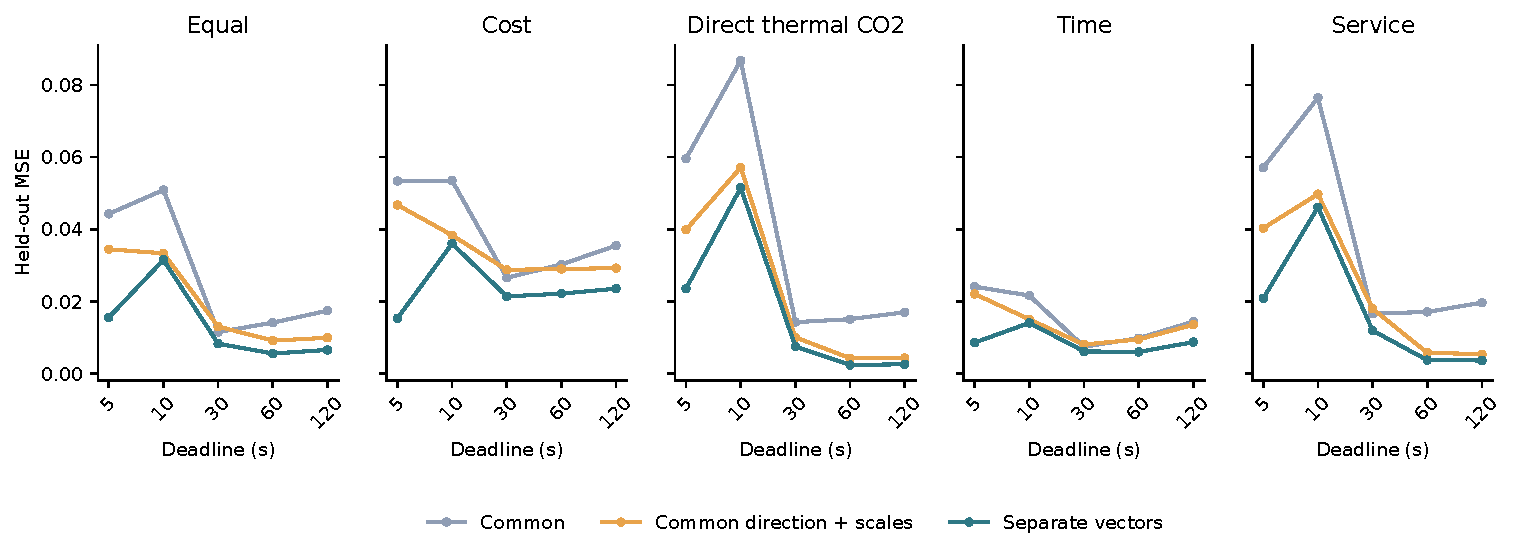
\includegraphics[width=\linewidth]{paper1/results/revision_scale_direction.pdf}\caption{Separating amplitude and direction changes using independent deadline-specific observations.}\end{figure}

\subsection{How much representation is necessary?}

\label{sec:revision_compact}

The 22-component separate model improves on B1 alone and on B1+B3+B4 for each pooled preference, but the flexible boosting model is more accurate for all five. The linear index is therefore an interpretability--accuracy compromise. Removing training-fold constants and correlations above 0.95 produces nearly unchanged losses; this is evidence against treating all 22 entries as distinct empirically identified dimensions. Fixed grouping of (A2,A4), (A3,A5) and (A7,A8), and a separate nonsaturating transformation of A6 and B8 are reported in the reproducibility tables. These are evaluated alternative representations, not silent changes to the historical index.

\subsection{What is predicted: delivery, quality or service?}

\label{sec:revision_failures}

At 5 seconds, 468 of 600 runs do not deliver a valid dispatch on time, 28 deliver but fail economic quality, and 3 pass economics but fail service. At 120 seconds, all deliver, 95 fail economics and 30 additional runs fail service. This decomposition separates pipeline delivery difficulty from the quality of a delivered dispatch (Figure~\ref{fig:revision_failures}).

\begin{figure}[htbp]\centering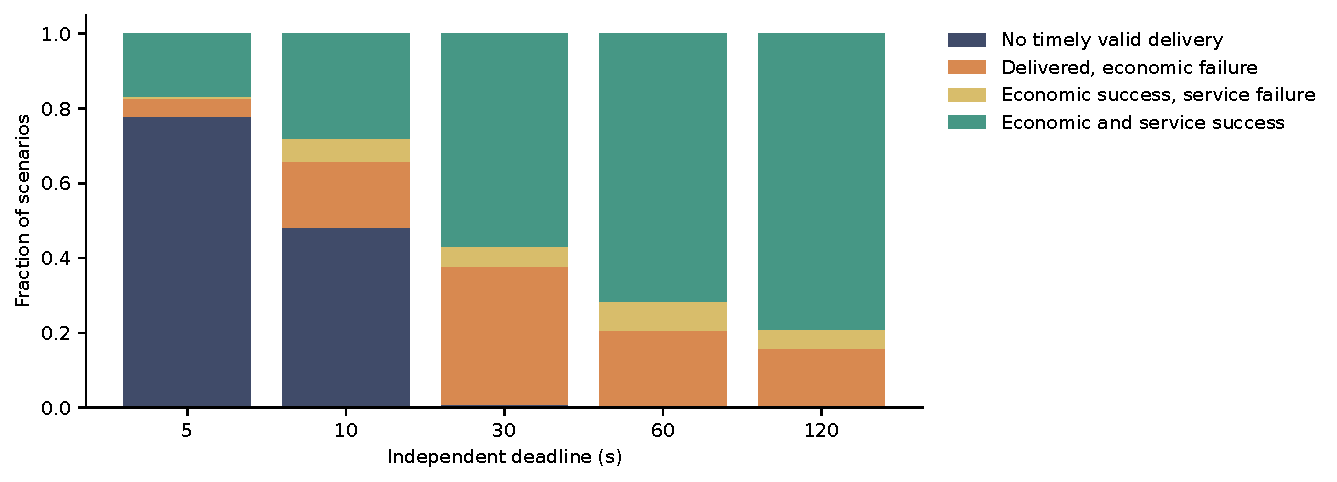
\includegraphics[width=.94\linewidth]{paper1/results/revision_failure_decomposition.pdf}\caption{Mutually exclusive observed outcomes. Short deadlines predominantly assess delivery of the complete computational pipeline.}\label{fig:revision_failures}\end{figure}

Conditional fractional-logistic fits estimate delivery, economic success given delivery, and service given economic success. Shared tuning of the conditional factors guarantees $\widehat P(ES)\leq\widehat P(E)$. A continuous two-part model combines non-delivery probability with the conditional bounded loss. Projection of linear predictions onto $[0,1]$ is also reported; it cannot increase squared error for this target. Calibration bins and their counts are included in the supplement.

\subsection{How far do the findings transfer?}

\label{sec:revision_transfer}

Leaving one complete family out, with leave-one-family-out tuning among the remaining five, reveals substantial deterioration. Family labels are excluded from all predictors. This assesses transfer among the six constructed regimes, not an independent external system.

\begin{table}[htbp]\centering\small\begin{tabular}{lrrr}\toprule Preference & Within-family folds & Held-out family & Ratio\\\midrule

Equal & 0.01353 & 0.04310 & 3.19\\

Cost & 0.02371 & 0.08601 & 3.63\\

Direct thermal CO$_2$ & 0.01753 & 0.04771 & 2.72\\

Time & 0.00873 & 0.03158 & 3.62\\

Service & 0.01728 & 0.05152 & 2.98\\

\bottomrule\end{tabular}\caption{Pooled MSE of separate 22-component models under the two validation designs. Ratios describe the change of evaluation distribution; they are not paired causal effects.}\label{tab:revision_transfer}\end{table}

The independent physical campaign is in progress: four batches of 100 fresh scenarios cover unfiltered draws, temporal structure, topology and decoupled parameters. Its predictors were frozen before execution and remain unchanged. No independent performance estimate is reported here (Section~\ref{sec:evidence_status}). Horizon coefficients remain unidentified in the historical training population.

\subsection{Can the descriptors improve a time-allocation decision?}

\label{sec:revision_allocation}

Within each outer test fold, an exact multiple-choice budget allocation maximizes predicted ES success subject to a sum of reserved deadlines. The model has seen none of the scenarios in that portfolio. E is a secondary endpoint. Uniform allocations, a predetermined adjacent-deadline mixture, size-only predictions, the original index, B1+B3+B4 and the observed-outcome oracle use the same budget constraint.

\begin{table}[htbp]\centering\small\begin{tabular}{rrrrrrr}\toprule Mean seconds & Uniform & Size & Index & Compact & 22 & Oracle\\\midrule

10 & 168 & 231 & 218 & 256 & 249 & 273\\

20 & 265 & 344 & 322 & 364 & 359 & 417\\

30 & 341 & 395 & 378 & 413 & 415 & 472\\

60 & 430 & 451 & 450 & 464 & 459 & 475\\

\bottomrule\end{tabular}\caption{Observed ES successes across five disjoint test portfolios, totaling 600 scenarios. The oracle uses observed outcomes, not true success probabilities.}\label{tab:revision_allocation}\end{table}

The compact representation matches or exceeds the 22-component allocation at three of the four budgets, despite its higher continuous prediction loss. Predictive accuracy and decision utility therefore yield different representation choices. Portfolio bootstrap intervals resample scenarios and reoptimize the allocation within each fold; models remain fixed. Reserved seconds and observed process-exit seconds are recorded separately. No observed portfolio exceeds its total reserve, but these retrospective sums do not establish a strict real-time guarantee or include the online cost of feature computation and allocation.

\begin{figure}[htbp]\centering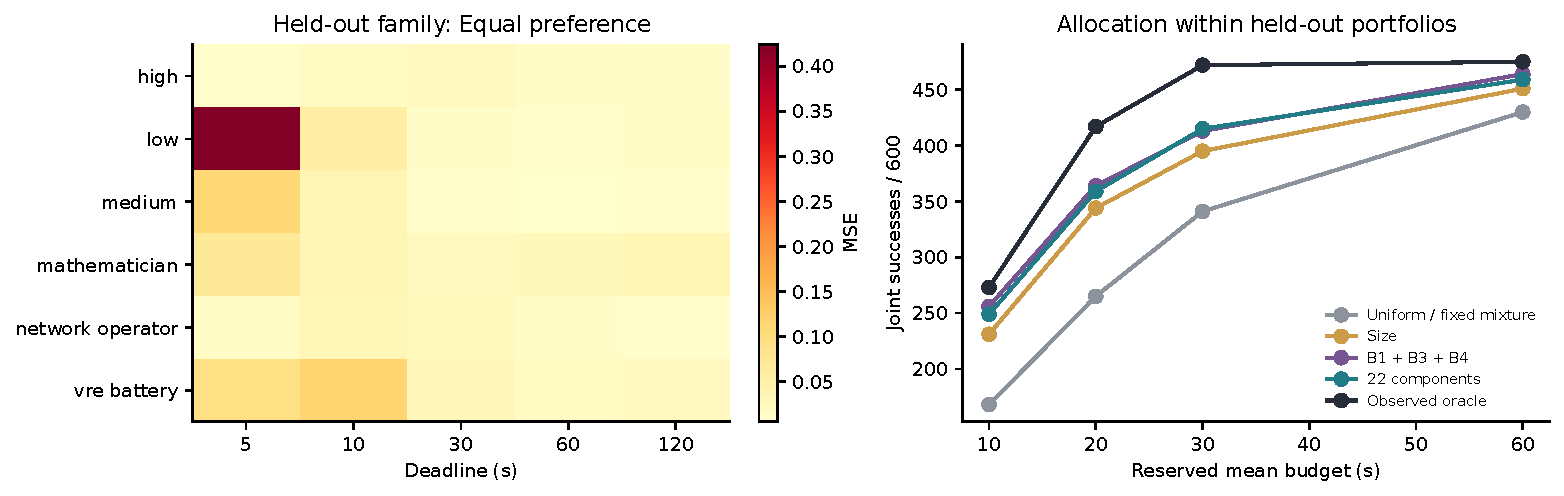
\includegraphics[width=\linewidth]{paper1/results/revision_transfer_allocation.pdf}\caption{Family transfer for the equal preference (left) and retrospective ES budget allocation (right). Predictive generalization is limited while within-regime decision utility can remain useful.}\end{figure}
